\chapter{Process optimization}
\label{chp:optimization}
Process optimization bears great potential for designing ecologically and economically optimal processes. 
Within this chapter first some basic concepts of constrained optimization are summarized as this proves 
useful for the remainder of the chapter. The problems arising when optimizing chemical processes involve 
both continuous and discrete decisions. In order to solve this class of so called mixed-integer non-linear
problems (MINLP) designated algorithms have to be employed to accommodate the special nature of the integer 
variables. The major approaches used today to solve this class of program  are summarized in the second section. 
Lastly these approaches be applied to several problems in the context of optimizing the cryogenic air separation 
process.
 
    \section{Optimization theory}
    \label{sec:opt:theory}
    The purpose of this section is not an exhaustive review of (convex) optimization but rather to mention
some elementary concepts and terms that will prove useful in the following sections. Initially optimality
conditions for constrained problems -- the so called Karush-Kuhn-Tucker (KKT)
conditions -- are briefly discussed. Closely linked to those conditions are the constraint qualifications, 
which are subsequently discussed.

    \subsection{Karush-Kuhn-Tucker conditions}
    \label{sec:opt:theory:kkt}
    This formulation of the KKT conditions is adapted from explanations in \cite{Nocedal.2006}.
    Before the conditions ca be stated, some definitions are needed. Considering the most general case of a NLP
    \program{}{
        & \minimize{x} & & f(x) \\
        & \st & & h_i(x) = 0, \; \; i \in \mathset{E} \\
        & & & g_i(x) \leq 0, \; \; i \in \mathset{I}
    }
    where $f(x): \mathbb{R}^n \mapsto \mathbb{R}$ denotes the objective function, $\mathset{E}$ and $\mathset{I}$
    are sets of indices corresponding to equality and inequality constraints respectively.
    the functions $f, g$ and $h$ are assumed to be differentiable and real-valued.

    The active set denotes the union of the set of equality constraints and the inequality constraints
    where $g_i(x) = 0$ holds. Thus we can write for the active set at any feasible point $x$
    \Eq{}{
       \mathset{A}(x) = \mathset{E} \cup \left\{ i \in \mathset{I} | g_i(x) = 0 \right\}.
    }

    For the constrained problem stated above the Lagrangian is defined as
    \Eq{}{
        \mathset{L}(x,\lambda,\mu) := f(x) - \sum_{i \in \mathset{E}} \lambda_i h_i(x) - \sum_{i \in \mathcal{I}} \mu_i g_i(x)
    }

    With that the optimality conditions for constrained optimization can be stated.
    First order or necessary KKT conditions must hold at the optimal point $(x^{\ast}, \lambda^{\ast}, \mu^{\ast})$
    \Eq{}{
        \nabla_x \mathcal{L}(x^{\ast}, \lambda^{\ast}, \mu^{\ast}) & = 0, \\
        h_i(x^{\ast}) & = 0, & \forall i \in \mathset{E} \\
        g_i(x^{\ast}) & \leq 0, & \forall i \in \mathset{I} \\
        \mu_i^{\ast} & \geq 0, & \forall i \in \mathset{I} \\
        \mu_i^{\ast} g_i(x^{\ast})& = 0, & \forall i \in \mathset{I} \\
        \lambda_i^{\ast} h_i(x^{\ast})& = 0, & \forall i \in \mathset{E}
    }
    The second order or sufficient KKT conditions can be written as
    \todo{check conditions on lagrange multipliers and active set ....}
    \Eq{}{
        w^T \nabla_{xx} \mathcal{L}(x^{\ast}, \lambda^{\ast}, \mu^{\ast})w & > 0, \quad \forall w \neq 0, \\
        \nabla h_i(x^{\ast})^T w & = 0, \quad \forall \; i \in \mathset{E}, \\
        \nabla g_i(x^{\ast})^T w & = 0, \quad \forall \; i \in \mathset{A}(x^{\ast}) \cap \mathset{I}, \; \text{with} \; \mu_i^{\ast} > 0 \\
        \nabla g_i(x^{\ast})^T w & \geq 0, \quad \forall \; i \in \mathset{A}(x^{\ast}) \cap \mathset{I}, \; \text{with} \; \mu_i^{\ast} = 0
    }

    \subsection{Constraint qualifications}
    \label{sec:opt:theory:cq}

    Constraint qualifications are used in the derivation of the optimality conditions. In the form presented here, 
    they are derived from the so call linear-independence constraint qualification. The derivation of 
    optimality conditions relies on approximating the objective function as well as the constraints by a 
    first order Taylor expansion. However there is no insurance that this linear model is in fact 
    an adequate representation of the original model around any given point. To resolve this issue, constraint 
    qualifications are used, to ensure, that the approximative model yields a similar representation of the 
    original one \cite{Nocedal.2006}. The significance of constraint qualifications in the context of this thesis, lies in a later 
    presented solution approach to mixed integer non-linear programs. 

    There are several constraint qualifications proposed in literature, which are differently hard to fulfil
    and verify. In general a minimum point should satisfy some constraint qualifications or regularity conditions.
    Among the most common qualifications are Slater's- (SCQ), linear independence- (LICQ) and the Mangasarian-Fromovitz (MFCQ)
    constraint qualification which are state here. Several more constraint qualifications can be found in literature, 
    but will not be stated here.

    \subsubsection{Slater's constraint qualification (SCQ)}
    Among the most widely used constraint qualifications is Slater's constraint qualification
    \Eq{}{
        \exists \tilde{x}, \forall i \in \mathcal{I} : h_i(\tilde{x}) < 0.
    }
    The main advantage of the SCQ is that the actual optimal point needs not to be known for checking
    if the SCQ is fulfilled.

    \subsubsection{Linear independence constraint qualification (LICQ)}
    Another widely used is called the linear independence constraint qualification. It states,
    given the set of of feasible solutions of the original problem $\mathcal{C} = \{x \in \mathcal{X} \; | \; h_i(x) \leq 0
    \forall i \in \mathcal{I} \}$ and the set of active constraints $\mathcal{A}(\bar{x}) = \{i \in \mathcal{i} \; | \; h_i(\bar{x}) = 0 \}$
    \Eq{}{
        \{ \nabla h_i(\bar{x}) \; | \; i \in \mathcal{A}(\bar{x}) \} \qquad \text{is linearly independent}.
    }

    \subsubsection{Mangasarian-Fromovitz constraint qualification (MFCQ)}
    \Eq{}{
        \exists \tilde{u}, \forall i \in \mathcal{A}(\bar{x}) : \nabla h_i(\bar{x})(\tilde{u}) < 0.
    }





    \section{Mixed-integer optimization}
    \label{sec:opt:MINLP}
    
In this section some general considerations about mixed-integer non-linear programming (MINLP) will be presented.
First the most commonly applied solution techniques will briefly be discussed on the basis of a review on the
subject by Grossmann \cite{Grossmann.2002}. Then then an alternative approach to solve this class of problems,
based on a continuous reformulation of the discrete decision variables, which has recently been proposed
\cite{Kraemer.2010,Stein.2004} will also be introduced. This reformulation is also the basis for a comparison of different
approaches to solve this class of problem within the process simulation environment \gproms.

    \subsection{Solution techniques}

    As previously stated, the following discussion of general solution techniques for MINLP's is largely based
    in the comprehensive review by I. E. Grossmann \cite{Grossmann.2002}.

    Several approaches to tackle this type of problem have successfully been applied to a multitude of cases for
    several years now. In general four major types of solution algorithms can be distinguished.
    \begin{itemize}
        \item branch and bound
        \item outer approximation
        \item generalized benders
        \item extended cutting plane
        \item LP/NLP ...
    \end{itemize}
    All these algorithms make use of a limited number of common subproblems, which are then solved
    in different configurations. Therefore these subproblems can previously be discussed and will be referred
    to when going elaborating on different algorithms. Furthermore it needs to be emphasised, that the presented
    solution techniques are designed for convex problems, and only in those cases an optimal solution can
    be found with a degree of confidence. While they can be applied to the more general non-convex case, only
    local optimality can be assured.

    The general case of a MINLP takes the form
    \program{prog:stdMINLP}{
        & \minimize{x,y} & & C = f(x,y) \\
        & \st & & g_j(x,y) \leq 0, \; \; j \in \mathset{J} \\
        & & & x \in \mathset{X}, \; y \in \mathset{Y}
    }

    If the discrete variables in the discrete-continuous program are relaxed, the resulting NLP relaxation
    can be written as
    \program{prog:relaxedNLP}{
        & \minimize{x,y} & & C_{LB}^k = f(x,y) \\
        & \st & & g_j(x,y) \leq 0, \; \; j \in \mathset{J} \\
        & & & x \in \mathset{X}, \; \; y \in \mathset{Y}_R \\
        & & & y_i \leq \alpha_i^k, \; i \in \mathset{I}_{FL}^k \\
        & & & y_i \geq \beta_i^k, \; i \in \mathset{I}_{FU}^k
    }
    Here $\mathset{Y}_R$ denotes the relaxed set of the integer set $\mathset{Y}$, $\mathset{I}_{FL}^k$ and
    $\mathset{I}_{FU}^k$ are subsets of the indices denoting the entire set of integer variables.
    The relaxed integers contained in these sets are  bounded to the values $\alpha_i^k$ and $\beta_i^k$ respectively.
    These bounds are lower and upper bound taken from the previous iteration of the algorithm in question. If
    $\mathset{I}_{FL}^k = \emptyset$ and $\mathset{I}_{FU}^k = \emptyset$ are empty sets, problem \progref{prog:relaxedNLP}
    denotes the fully relaxed problem, initially solved in all algorithms. The optimal solution to this initially solved
    problem ($C_{LB}^0$) poses an absolute lower bound to \progref{prog:stdMINLP} since all variables are fully relaxed.

    If all discrete variables are fixed at a given value, the NLP subproblem for fixed $y^k$ results, as
    only continuous variables are being considered.
    \program{prog:fixedyNLP}{
        & \minimize{x} & & C_{LB}^k = f(x,y^k) \\
        & \st & & g_j(x,y^k) \leq 0, \; \; j \in \mathset{J} \\
        & & & x \in \mathset{X}
    }
    If \progref{prog:fixedyNLP} is infeasible the NLP feasibility subproblem for fixed $y^k$ can be solved.
    \program{prog:feasibleNLP}{
        & \minimize{x} & & u \\
        & \st & & g_j(x,y^k) \leq u, \; \; j \in \mathset{J} \\
        & & & x \in \mathset{X}, \; \; u \in \mathbb{R}
    }
    This NLP returns a strictly positive value for $u$.

    Aside from the presented NLP's a linearized version of \progref{prog:stdMINLP} is regularly solved
    \program{prog:MILP}{
        & \minimize{x, y} & & C_L^k = \alpha \\
        & \st & & f(x^k,y^k) + \nabla f(x^k,y^k)^T \begin{bmatrix} x - x^k \\ y - y^k \end{bmatrix} \leq \alpha \\
        & & & g_j(x^k,y^k) + \nabla g_j(x^k,y^k)^T \begin{bmatrix} x - x^k \\ y - y^k \end{bmatrix} \leq 0, \; \; j \in \mathset{J} \\
        & & & x \in \mathset{X}, \; \; y \in \mathset{Y}, \; \; k = {1 \dots K}
    }
    The linearized problem can be constructed in several ways from the set of points $K$ attained in previous iterations.
    Sometimes only violated or active constraints are linearized. When objective function and constraints are convex, the
    objective function is underestimated, while the constraints are overestimated. From the overestimated constraints stems
    the name outer approximation.

        \subsubsection{Branch \& bound (B\&B)}
        The branch and bound (B\&B) algorithm has originally been proposed for linear problems, but has since been extended to
        handle non-linear objectives and constraints. As an initial step for the branch and bound the fully relaxed
        NLP \progref{prog:relaxedNLP} is solved, which, as mentioned before, provides an absolute lower bound to
        the program in question. In the rare case that all relaxed integer variables assume integer values the optimal
        solution has been found and the algorithm can terminate. Otherwise a tree search is performed, exploring the
        space of the integer variables. In each step an increasing number of integer variables is fixed such that
        a NLP in the form of \progref{prog:fixedyNLP} needs to be solved. The solution of these subproblems is
        a new lower bound for all descendant nodes. Further exploration of branches can be stopped, once a
        given subproblem returns a value grater than the current upper bound or becomes infeasible.

        Due to the large number of NLP subproblems that have to be solved within the tree search, the branch and bound
        algorithm is most attractive, if the solution is computationally inexpensive, or few nodes have to be explored.

        \subsubsection{Outer approximation (OA)}
        The outer approximation (OA) algorithm relies on consecutively solving \progref{prog:fixedyNLP} and
        \progref{prog:MILP}. Each solution of the NLP with fixed $y^k$ yields a new point $(x^k,y^k)$ which is used to
        construct an updated version of the MILP. The MILP generally includes linearized versions of all constraints and
        the objective function. As more and more points become available during the iterative process, new constraints
        are constructed for each available point.

        The main theorem for the derivation of the OA algorithm states, that the optimal solution of the problem
        \progref{prog:MILP} constructed from all points $(x^k,y^k), k \in K^{\ast}$. Where $K^{\ast}$ is made up of
        all optimal solutions of \progref{prog:fixedyNLP} where the current $y^k$ yields a feasible solution, and
        \progref{prog:feasibleNLP} where infeasible solutions of the NLP with fixed $y^k$ are encountered. It should
        again be emphasized, that this theorem holds only for convex a objective function and constraints.

        As the points necessary to construct the aforementioned system are not available when the solution process
        commences, a smaller systems is constructed and extended as more points become available. The first point again
        results from solving a fully relaxed system. \todo{is this true, that the fully relaxed system is initially
        solved????} This again yields an absolute lower bound for the original problem. The solution of each consecutive
        MILP gives a new lower bound which will always be greater than the bounds from previous iterations. Without any
        prove this argument is supported by the fact that adding new linear constraints will limit the feasible region of
        the problem and hence further restrict the possible solutions for the continuous variables.

        The optimal points attained from the NLP subproblems with fixed discrete values form upper bounds on the optimal
        solution. Here no statement can be made about the quality of the bound in each step, but rather is the current
        upper bound updated, once a lower value is encountered.

        The iterative process terminates, once the current upper and lower bound are within a given tolerance. It can be
        pointed out, that the outer approximation algorithm converges to the optimal solution in a single iteration if
        objective function and constraints in the original problem are linear, since in that case problems
        \progref{prog:stdMINLP} and \progref{prog:MILP} are equivalent.

        \subsubsection{Generalized Benders decomposition (GBD)}
        The generalized Benders decomposition is very similar to the outer approximation algorithm. The main difference
        lies in way that \progref{prog:MILP} is constructed. While for the outer approximation problem all constraints
        are included, in case of the GBD only active constraints are $J^k = \{j \; | \; g_j(x^k,y^k) = 0\}$ considered.
        Furthermore the set of continuous variables is eliminated by considering the KKT-conditions. The resulting problem
        \program{}{
            & \minimize{y} & & C^K_L = \alpha \\
            & \st & & f(x^k,y^k) + \nabla_y f(x^k,y^k)^T (y - y^k) \\
            & & & \; \;  + (\mu^k)^T \left[ g(x^k,y^k) + \nabla_y g(x^k,y^k)^T (y - y^k) \right] \leq \alpha, \; \; k \in \mathcal{K}_{FS} \\
            & & & (\lambda^k)^T \left[ g(x^k,y^k) + \nabla_y g(x^k,y^k)^T (y - y^k) \right] \leq 0, \; \; k \in \mathcal{K}_{IS} .
        }
        Where $\mathcal{K}_{FS}$ and $\mathcal{K}_{IS}$ denote the sets of solutions for of feasible and infeasible
        iterations respectively.

        This difference in formulation the MILP in the OA and GBD algorithm is what leads to the major computational differences.
        In general the MILP in the OA algorithm is expected to return tighter bounds than the respective
        problem in GBD. However the computational effort to solve the problem might be considerably higher for the
        OA case. Hence the GBD is expected to need more iterations, before converging, while the cost of a single
        iteration might be lower.

        \subsubsection{Extended cutting plane (ECP)}
        The extended cutting plane method requires no solution any NLP subproblems. Rather a version of the linearized
        problem is solved during each iteration. After each iteration the problem is extended by an addition cut or
        linearized constraint. Most commonly a linear version of the most violated constraint is added. A further
        possibility is to add all violated constraints to the problem. It should be noted, that for the ECP method
        the objective function has to be linear. If necessary non-linearities in the objective function can be moved to the
        constraints by introduction of new variables.

        \subsubsection{LP/NLP branch \& bound}



    \subsection{Continuous reformulation}
    \label{sec:opt:theory:continuous}
    An alternative approach to solving discrete-continuous problems is to reformulate them as NLP
    and introduce further constraints which ensure that the discrete decision variables will assume integer values.
    Several different authors have proposed ways of reformulating integer decisions. The concept of continuous reformulation
    will be discussed with the current example of the ASU process in mind. First an approach using 
    
        \subsubsection{Non-linear complementary problem (NCP / MECP)}
        The following discussion is modeled on the remarks of the topic in \cite{Stein.2004} and fitted to the case under consideration.
    
%        In the context of a column model, all decisions regarding feed and side draw locations as well as the minimum number
%        of trays can be seen as \emph{exclusive or} decisions, as the the stream can only be fed to or drawn from exactly one
%        stage. This can be expressed in the integer case by adding the constraint
%        \Eq{}{
%            & \sum_{j}^{n_S} y_{j,k} = 1 \\
%            & y_{j,k} \in \{0,1\}, \; \; k \in \mathcal{K}.
%        }
%        to the model equations. Here again $j$ denotes the number of stages and $\mathcal{K}$ is the set of decisions to be made,
%        corresponding to feed and side draw locations as well as the number of trays in a column.
%    
%        If one defines a set $\mathcal{A}_0 = \{(1,0), (0,1)\}$ the summation constraint given earlier can be dropped
%        \Eq{}{
%            \left( y_{i,k}, \sum_{\genfrac{}{}{0pt}{}{j}{j \neq i}}^{n_S} y_{j} \right) \in \mathcal{A}_0, \eqannote{k \in \mathcal{K}}.
%        }
        Several approaches can be found in literature as to how discrete-continuous problem can be reformulated. For an overview of alternatives
        the reader is referred to \cite{Stein.2004}. In many cases these reformulations lead to numerically difficult programs and 
        unattractive theoretical properties. The aforementioned constraint qualifications are often violated.  
    
        \begin{figure}
            \scriptsize
            \center
            % GNUPLOT: LaTeX picture with Postscript
\begingroup
  \makeatletter
  \providecommand\color[2][]{%
    \GenericError{(gnuplot) \space\space\space\@spaces}{%
      Package color not loaded in conjunction with
      terminal option `colourtext'%
    }{See the gnuplot documentation for explanation.%
    }{Either use 'blacktext' in gnuplot or load the package
      color.sty in LaTeX.}%
    \renewcommand\color[2][]{}%
  }%
  \providecommand\includegraphics[2][]{%
    \GenericError{(gnuplot) \space\space\space\@spaces}{%
      Package graphicx or graphics not loaded%
    }{See the gnuplot documentation for explanation.%
    }{The gnuplot epslatex terminal needs graphicx.sty or graphics.sty.}%
    \renewcommand\includegraphics[2][]{}%
  }%
  \providecommand\rotatebox[2]{#2}%
  \@ifundefined{ifGPcolor}{%
    \newif\ifGPcolor
    \GPcolortrue
  }{}%
  \@ifundefined{ifGPblacktext}{%
    \newif\ifGPblacktext
    \GPblacktexttrue
  }{}%
  % define a \g@addto@macro without @ in the name:
  \let\gplgaddtomacro\g@addto@macro
  % define empty templates for all commands taking text:
  \gdef\gplbacktext{}%
  \gdef\gplfronttext{}%
  \makeatother
  \ifGPblacktext
    % no textcolor at all
    \def\colorrgb#1{}%
    \def\colorgray#1{}%
  \else
    % gray or color?
    \ifGPcolor
      \def\colorrgb#1{\color[rgb]{#1}}%
      \def\colorgray#1{\color[gray]{#1}}%
      \expandafter\def\csname LTw\endcsname{\color{white}}%
      \expandafter\def\csname LTb\endcsname{\color{black}}%
      \expandafter\def\csname LTa\endcsname{\color{black}}%
      \expandafter\def\csname LT0\endcsname{\color[rgb]{1,0,0}}%
      \expandafter\def\csname LT1\endcsname{\color[rgb]{0,1,0}}%
      \expandafter\def\csname LT2\endcsname{\color[rgb]{0,0,1}}%
      \expandafter\def\csname LT3\endcsname{\color[rgb]{1,0,1}}%
      \expandafter\def\csname LT4\endcsname{\color[rgb]{0,1,1}}%
      \expandafter\def\csname LT5\endcsname{\color[rgb]{1,1,0}}%
      \expandafter\def\csname LT6\endcsname{\color[rgb]{0,0,0}}%
      \expandafter\def\csname LT7\endcsname{\color[rgb]{1,0.3,0}}%
      \expandafter\def\csname LT8\endcsname{\color[rgb]{0.5,0.5,0.5}}%
    \else
      % gray
      \def\colorrgb#1{\color{black}}%
      \def\colorgray#1{\color[gray]{#1}}%
      \expandafter\def\csname LTw\endcsname{\color{white}}%
      \expandafter\def\csname LTb\endcsname{\color{black}}%
      \expandafter\def\csname LTa\endcsname{\color{black}}%
      \expandafter\def\csname LT0\endcsname{\color{black}}%
      \expandafter\def\csname LT1\endcsname{\color{black}}%
      \expandafter\def\csname LT2\endcsname{\color{black}}%
      \expandafter\def\csname LT3\endcsname{\color{black}}%
      \expandafter\def\csname LT4\endcsname{\color{black}}%
      \expandafter\def\csname LT5\endcsname{\color{black}}%
      \expandafter\def\csname LT6\endcsname{\color{black}}%
      \expandafter\def\csname LT7\endcsname{\color{black}}%
      \expandafter\def\csname LT8\endcsname{\color{black}}%
    \fi
  \fi
  \setlength{\unitlength}{0.0500bp}%
  \begin{picture}(4762.00,1926.00)%
    \gplgaddtomacro\gplbacktext{%
      \csname LTb\endcsname%
      \put(686,320){\makebox(0,0)[r]{\strut{} 0.0}}%
      \put(686,1027){\makebox(0,0)[r]{\strut{} 0.2}}%
      \put(686,1200){\makebox(0,0)[r]{\strut{} $\mu$}}%
      \put(686,1733){\makebox(0,0)[r]{\strut{} 0.4}}%
      \put(782,160){\makebox(0,0){\strut{} 0.0}}%
      \put(1489,160){\makebox(0,0){\strut{} 0.2}}%
      \put(2195,160){\makebox(0,0){\strut{} 0.4}}%
      \put(2902,160){\makebox(0,0){\strut{} 0.6}}%
      \put(3608,160){\makebox(0,0){\strut{} 0.8}}%
      \put(4315,160){\makebox(0,0){\strut{} 1.0}}%
    }%
    \gplgaddtomacro\gplfronttext{%
    }%
    \gplbacktext
    \put(0,0){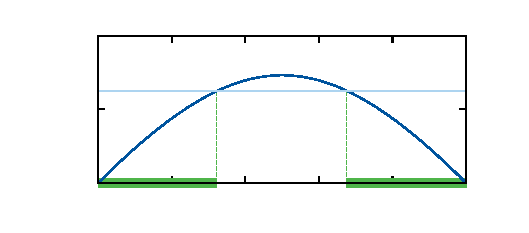
\includegraphics{GNUPlot/FB_Plot}}%
    \gplfronttext
  \end{picture}%
\endgroup

            \caption{plot of Fischer-Burmeister function.}
            \label{fig:FB_plot}
        \end{figure}
    
        To arrive at a formulation with favourable theoretical properties Kraemer et al. \cite{Kraemer.2009} proposed
        a continuous reformulation based on the Fischer-Burmeister nonlinear complementary problem (NCP) - function
        \Eq{eq:opt:FB}{
            1 - \sqrt{y_i^2 + (1 - y_i)^2} = 0.
        }
        If this function has exactly the values zero and one as solutions and hence forces a continuous variable to
        take integer values. However it is still very hard to solve complex, large-scale problems by simply enforcing this
        constraint. In order to facilitate convergence, the FB-function can be relaxed to a fully continuous problem
        \Eq{eq:opt:FB}{
            1 - \sqrt{y_i^2 + (1 - y_i)^2} \leq \mu.
        }
        The relaxation factor $\mu$ is then gradually reduced to zero in a sequence of NLP problems. \Figref{fig:FB_plot}
        shows a plot of the FB-function over the domain zero to one. The green lines on the x-axis denote the feasible domain
        for a given value of $\mu$. As one can see, if the relaxation factor is chosen large enough the entire span
        between zero and one is feasible.
    
        \subsubsection{Differentiable distribution function (DDF)}
        An alternative way of reaching a continuous formulation was brought fourth by Lang and Biegler \cite{Lang.2002}
        who propose the introduction of a differentiable distribution function (DDF)
        \Eq{}{
            \Psi_j = \frac{ \exp\left[ - \left( \frac{j - \sum_i \zeta_i i}{\sigma} \right)^2 \right] }{
                \sum_k \exp\left[ - \left( \frac{k - \sum_i \zeta_i i}{\sigma} \right)^2 \right]}.
        } 
        

    \section{Optimization examples}
    \label{sec:opt:apllication}
    The simulation of chemical processes supplies valuable insight into the intricacies of a given system. 
To some extend it is also possible to improve given designs by manual alterations and simulation
steps in a form of trial an error procedure. However the results of an approach like that are unlikely 
to yield even locally optimal results in an acceptable amount of time. Hence optimization approaches
are employed to attain improved designs. 

The models presented in the previous chapters are capable of projecting various continuous and 
discrete design decisions. However when synthesizing a process flowsheet, one must take careful 
consideration as to the optimization objectives. The most obvious objective would be of 
pure monetary nature, where a process is designed to meet a given set of specifications 
at minimum cost. An optimization like that can be carried out at steady state. However for
a steady state model it is never ensured, that this steady state can actually be reached 
by the process. Furthermore is there no consideration if the desired steady state can be kept for
changing conditions outside the control of the process operator. 

In the case that load changes or different operation modes are required, it becomes questionable, 
if steady state optimization remains feasible, or if a dynamic approach becomes necessary. 

In this chapter different optimization studies will be given. For once different solution approaches 
will be applied to the MINLP arising from a steady state simulation. For once the outer approximation 
algorithm as implemented in \gproms, and secondly the continuous reformulation strategy as described 
in \Secref{sec:opt:theory:continuous}. 

The process under consideration is a generic cryogenic air separation process. As a starting point for the 
optimization a base case was manually constructed which met certain somewhat arbitrarily chosen, 
but reasonable constraints.  

\todo{describe reference case.}

    \subsection{Degrees of freedom}
    \todo{move to description of dynamic model.}
    In order to gain more insight into the behaviour of the dynamic models presented above an analysis
    of the degrees of freedom within the model is at hand. For the degrees of freedom the cost correlations
    will be disregarded, as they for a closed system of equations given the inputs generated form the column
    model. Furthermore interdependencies can be disregarded, as the cost model consist only of ''forward''
    computations. In practical terms this statement can be confirmed since the models can be evaluated
    with and without costing equations. Hence only the stage and hydraulic equations will be considered.

    For a given column without condenser or reboiler the model is made up of $[n_S (5n_C + 24) + n_F]$
    differential algebraic equations in $[n_S (5n_C + 29) + n_F (n_S + n_C + 3) + 1]$ variables. In this
    isolated case all feed flow rates, their composition and enthalpies would be specified. In this case
    the feeds include a hypothetical condenser reflux (the upper most feed) as well as reboiler reflux
    (lowest feed). Along with the feeds and their qualities, the feed splits and reflux split have to be
    assigned. Lastly the column diameter needs to be known. This yields $[n_F (n_S + n_C + 2) + n_S + 1]$
    specifications. To close the system initial conditions for all states have to be given. There
    are a total of $[4 n_S ]$ dynamic stages in a column section.

    The condenser reboiler unit

    \subsection{Steady state single period}
    \label{chp:optexample:ss_single_perid}
    Objective function
    \Eqml{eq:opt:ss_single_objective}{
        CAPEX = \left( \sum_c C_c^{\text{cap}} \right) \cdot \left(q^{-a} \frac{q^a - 1}{q - 1} \right) + \sum_o C_o^{\text{oper}} \\
            \eqannote{c = \left\{ \text{HPC}, \text{LPC}, \text{CAC}, \text{HX}, \text{CP}, \text{CRM}, \text{CRCAC} \right\}
                \quad o = \left\{\text{CP}, \text{EXP} \right\}}
    }
    Constraints :
    Limits on the product purities:
    \Eq{eq:opt:ss_single_constraints_1}{
        y_{1,N_2}^{HPC} & \geq 0.985 \\
        y_{1,N_2}^{LPC} & \geq 0.985 \\
        y_{1,Ar}^{CAC} & \geq 0.985 \\
        x_{reb}^{CRM} & \geq 0.985
    }
    No flooding in the columns:
    \Eq{eq:opt:ss_single_constraints_2}{
        d_{\text{column}}^{\text{HPC}} & \geq d_{min}^{HPC} \\
        d_{\text{column}}^{\text{LPC}} & \geq d_{min}^{LPC} \\
        d_{\text{column}}^{\text{CAC}} & \geq d_{min}^{CAC}
    }
    No entrainment in the trayed column :
    \Eq{eq:opt:ss_single_constraints_3}{
        \left(1- \sum_{k=1}^{j-1} \right) ent_k^{HPC} & \leq 0.1
    }
    Limit on cooling water outlet temperatures to prevent corrosion :
    \Eq{eq:opt:ss_single_constraints_4}{
        T_{\text{w,out}}^{IC1} & \leq 323.15 \\
        T_{\text{w,out}}^{IC2} & \leq 323.15 \\
        T_{\text{w,out}}^{IC3} & \leq 323.15
    }

    Design Variables
    \begin{itemize}
        \item HPC diameter $d_{\text{column}}^{\text{HPC}}$
        \item LPC diameter $d_{\text{column}}^{\text{LPC}}$
        \item CAC diameter $d_{\text{column}}^{\text{CAC}}$
        \item HPC reflux location $\zeta^R_{\text{HPC}}$
        \item LPC reflux location $\zeta^R_{\text{LPC}}$
        \item CAC reflux location $\zeta^R_{\text{CAC}}$
        \item LPC CAC side draw location $\zeta^{SV,\text{LPC}}_{2,j}$
        \item heat exchange area multi-stream heat exchanger $A_{\text{HX}}^{multiHX}$
        \item heat exchange area main condenser reboiler $A_{\text{HX}}^{CRM}$
        \item heat exchange area CAC condenser reboiler $A_{\text{HX}}^{CRCAC}$
    \end{itemize}

    Manipulated Variables
    \begin{itemize}
        \item intercooler outlet temperatures ($T_{\text{out}}^{IC1}, T_{\text{out}}^{IC2}, T_{\text{out}}^{IC3}$)
        \item HPC dimensionless side draw (gaseous $N_2$product) ($s_1^{V, \text{HPC}}$)
        \item LPC dimensionless side draws ($s_i^{V, \text{LPC}}$)
    \end{itemize}

\subsection{Optimization \& control}
	To include the design of a PI control structure in the process, the following constraints need to be added.
	\Eq{}{
		u_m & = b_{m,1} + \sum_{j=1}^{n_m} \left( K_{m,n} \cdot e_{m,n} + I_{m,n} \right),
			\eqannote{m = 1 \dots n_{in}}, \\
		e_{m,n} & = set_{m,n} - meas_{n} \eqannote{m = 1 \dots n_{in}, n = 1 \dots n_m}, \\
		\frac{\mathrm{d} I}{\mathrm{d} t} & = \frac{e_{m,n}}{\tau_{m.n}} \eqannote{m = 1
			\dots n_{in}, n = 1 \dots n_m}, \\
		\frac{\mathrm{d} I}{\mathrm{d} t} & = 0 \eqannote{m = 1 \dots n_{in}, n = 1 \dots n_m}, \\
		set_{m,n} & = set_{m-1,n} \eqannote{m = 2 \dots n_{in}, n = 1 \dots n_m}, \\
		K^L_{m,n} \cdot \zeta^C_{m,n} & \leq K_{m,n}  \leq K^U_{m,n} \eqannote{m = 1 \dots n_{in},
			n = 1 \dots n_m}, \\
		\sum_{m=1}^{n_m} \zeta_{m,n}^C & = 1 \eqannote{m = 1 \dots n_{in}}, \\
		\sum_{n=1}^{n_{in}} \zeta_{m,n}^C & = 1 \eqannote{n = 1 \dots n_{m}},
	}
	Since new states have been introduced, the corresponding initial conditions will have to be included
	\Eq{}{
		I_{m,n} (t = 0) & = 0, \eqannote{m = 1 \dots n_{in}, n = 1 \dots n_m} \\
		e_{m,n} (t = 0) & = 0, \eqannote{m = 1 \dots n_{in}, n = 1 \dots n_m} \\
	}


